%%% File encoding is UTF8

%%% If you use this template then please give credit like this:
%%% ----------------------------
% LaTeX code inspired by the LaTeX Thesis Template by Manuel Kuehner 
% www.bedienhaptik.de/latex-template/
%%% ----------------------------

% ##############################################
% Start: Template Preamble
% ##############################################
%

% Documentclass definition
%%% File encoding is UTF8
%%% You can use special characters just like ä,ü and ñ

% KOMA-Script class 'scrbook'
% Link to the documentation: 
% German: http://mirrors.ctan.org/macros/latex/contrib/koma-script/doc/scrguide.pdf
% English: http://mirrors.ctan.org/macros/latex/contrib/koma-script/doc/scrguien.pdf
% CTAN: http://www.ctan.org/pkg/koma-script
% Author of the KOMA-Script family is Markus Kohm
\documentclass[paper=letter % Letter is "carta"
			 , fontsize=10pt % Arial 10 for all text.
			 , headings=big
			 , parskip=half-
			%, noparskip % No par skip. If yes park skip the command is parskip
			%, numbers=noendperiod % 2.3.1 vs 2.3.1. (no dot after the last chapter number)
			 , numbers=endperiod
	         , twoside=false
			% , toc=bibliography % Bibliography appears in Table of Contents (without a number)
			% , toc=listof % List of Figures and List of Tables appear in Table of Contents
			% , chapterprefix=true
			 , chapterprefix=false
			% , bibliography=totoc % The bibliography will have an entry at the table of contents but no number.
			 , numbers=noenddot
			 , titlepage=simple
			 , headings=onelinechapter
			 , version=last % Use latest version of the KOMA-Script
			 , final
]{scrbook}

\RedeclareSectionCommand[
afterskip=\parskip]{chapter}
\RedeclareSectionCommand[
beforeskip=\parskip
, afterskip=0.1\parskip]{section}
\RedeclareSectionCommand[
beforeskip=1.1\parskip plus 3mm
, afterskip=0.1\parskip]{subsection}


\KOMAoption{bibliography}{leveldown}

\newcommand{\mychapter}[1]{%
	\chapter{#1}
	\addcontentsline{lof}{chapter}{%
		Figuras del Capítulo \thechapter: #1 \vspace{10pt}
	}
}

\addtokomafont{section}{\large}
\addtokomafont{subsection}{\normalsize}  %1.1.1 Minus size: 10 % normalsize is 10

%REVISAR
\usepackage[compact]{titlesec}

% Titles in the chapters, not in TOC.
\titleformat{\chapter}
{\bfseries\Large\vspace*{-4.0cm}}	% Formato título
{	% Contenido de la etiqueta
	\filright
	\Large\MakeUppercase\chaptertitlename\ \thechapter.\ 
}
{0pt} % Espacio mínimo entre etiqueta y cuerpo
{\filright\MakeUppercase} % Código que precede al cuerpo del título
[\vspace{1.5pt}] % Margen de 1.5pt

\titleformat{\section}
{\bfseries\large\vspace{2pt}}
{\large\MakeUppercase\thesection\ \vspace{2pt} } % 3 espacios luego del titulo de una seccion
{0pt}
{\MakeUppercase}
[\vspace*{0.5cm}]

\titleformat{\subsection}
{\bfseries\normalsize\vspace{2pt}} % 3 espacios luego del titulo de una seccion
{\normalsize\thesubsection\ }
{0pt}
{\vspace*{0.5cm}}

\titleformat{\subsubsection}
{\itshape\normalsize\vspace{1.0cm}}
{\itshape\thesubsubsection\ }
{0pt}
{\vspace*{0.5cm}\itshape}

\titlespacing*{\chapter} {0pt}{85pt}{20pt} 
\titlespacing*{\section} {0pt}{6.5ex plus 1ex minus .2ex}{2.3ex plus .2ex}
\titlespacing*{\subsection} {0pt}{6.5ex plus 1ex minus .2ex}{2.3ex plus .2ex}
\titlespacing*{\subsubsection}{0pt}{3.25ex plus 1ex minus .2ex}{1.5ex plus .2ex}
\titlespacing*{\paragraph} {0pt}{3.25ex plus 1ex minus .2ex}{1em}
\titlespacing*{\subparagraph} {\parindent}{3.25ex plus 1ex minus .2ex}{1em}


% Loading additional packages from the KOMA-Script family
%%% File encoding is UTF8
%%% You can use special characters just like ä,ü and ñ

% Special KOMA-Script package - I added it because I also use the float package in this template, see: 
% http://tex.stackexchange.com/questions/51867/koma-warning-about-toc
% CTAN: http://www.ctan.org/tex-archive/macros/latex/contrib/koma-script/doc
\usepackage{scrhack}

% Better support for marginnotes
% new command: \marginnote
% LaTeX standard command: \marginpar
% CTAN: http://www.ctan.org/pkg/marginnote
\usepackage{marginnote}

% Extended header and footer support
% CTAN: http://www.ctan.org/pkg/scrpage2
\usepackage[automark
  		  , ilines
		  , headsepline
		  , footsepline
]{scrpage2}

\usepackage{setspace}
\onehalfspace

% Page layout definition
%%% File encoding is UTF8
%%% You can use special characters just like ä,ü and ñ

% User friendly interface to change layout parameters
% CTAN: http://www.ctan.org/pkg/geometry
\usepackage{geometry}
\geometry{%
	%bottom=30mm,
	, showframe=false % For debugging: try true and see the layout frames
	%, margin=30mm
	%, marginparsep=3mm
	%, marginparwidth=20mm
	, headheight=14pt
	, top=2.5cm
	, bottom=2.5cm 
	, left=4cm
	, right=2.5cm
	, letterpaper
}



% Standard packages
%%% File encoding is UTF8
%%% You can use special characters just like ä,ü and ñ

% Input encoding is 'latin1' (Latin 1 - also known as ISO-8859-1)
% CTAN: http://www.ctan.org/pkg/inputenc
% 
% A newer package is available - you may look into:
% \usepackage[x-iso-8859-1]{inputenc}
% CTAN: http://www.ctan.org/pkg/inputenx
%\usepackage[latin1]{inputenc}
\usepackage[utf8]{inputenc}

% Font Encoding is 'T1' -- important for special characters such as Umlaute ü or ä and special characters like ñ (enje)
% CTAN: http://www.ctan.org/pkg/fontenc
\usepackage[T1]{fontenc}

% Language support for 'english' (alternative 'ngerman' or 'french' for example)
% This case is in spanish
% CTAN: http://www.ctan.org/pkg/babel
%\usepackage[english]{babel} 
\usepackage[spanish
          , es-tabla
          , es-noindentfirst]{babel} 

% Doing calculations with LaTeX units -- needed for the vertical line in the footer
% CTAN: http://www.ctan.org/pkg/calc
\usepackage{calc}

% Extended graphics support 
% There is also a package named 'graphics' - watch out!
% CTAN: http://www.ctan.org/pkg/graphicx
\usepackage{graphicx}

% Extendes support for floating objects (tables, figures), adds the [H] placing option (\begin{figure}[H]) which palces it "Here" (without any doubt).
% CTAN: http://www.ctan.org/pkg/float
\usepackage{float}

% Extended color support
% I use the command \definecolor for example. 
% Option 'Table': Load the colortbl package, in order to use the tools for coloring rows, columns, and cells within tables.
% CTAN: http://www.ctan.org/pkg/xcolor
\usepackage[table]{xcolor} 

% Nice tables
% CTAN: http://www.ctan.org/pkg/booktabs
\usepackage{booktabs}

\usepackage{colortbl}

\usepackage{multirow,siunitx}

% Better support for ragged left and right. Provides the commands \RaggedRight and \RaggedLeft. 
% Standard LaTeX commands are \raggedright and \raggedleft
% http://www.ctan.org/pkg/ragged2e
\usepackage{ragged2e}

% Create function plots directly in LaTeX
% CTAN: http://www.ctan.org/pkg/pgfplots
\usepackage{pgfplots}
\pgfplotsset{compat=1.11}

% Main Font used: Arial
\usepackage{uarial}
\usepackage[expert]{mathdesign}
\renewcommand{\familydefault}{\sfdefault}

% tocloft ? Control table of contents, figures, etc
% CTAN: https://ctan.org/pkg/tocloft
%\usepackage{tocloft}

% Configure Microtype
\usepackage[activate={true,nocompatibility},final,tracking=true,kerning=true,spacing=true,factor=1100,stretch=10,shrink=10]{microtype}
% activate={true,nocompatibility} - activate protrusion and expansion
% final - enable microtype; use "draft" to disable
% tracking=true, kerning=true, spacing=true - activate these techniques
% factor=1100 - add 10% to the protrusion amount (default is 1000)
% stretch=10, shrink=10 - reduce stretchability/shrinkability (default is 20/20)

\SetExtraKerning[unit=space]
{encoding={*}, family={bch}, series={*}, size={footnotesize,small,normalsize}}
{\textendash={400,400}, % en-dash, add more space around it
	"28={ ,150}, % left bracket, add space from right
	"29={150, }, % right bracket, add space from left
	\textquotedblleft={ ,150}, % left quotation mark, space from right
	\textquotedblright={150, }} % right quotation mark, space from left

\SetExtraKerning[unit=space]
{encoding={*}, family={qhv}, series={b}, size={large,Large}}
{1={-200,-200}, 
	\textendash={400,400}}

% Use French spacing
\frenchspacing



% https://www.ctan.org/pkg/biblatex-ieee
\usepackage[backend=biber
		  %, style=ieee % Esta bien, pero no agrupa las citaciones
		  %, style=numeric-comp %Revisar, porque algunas referencias no las tira correctas
		  %Antes: IEEE
		  %, bibstyle=ieee  %Combinacion de ambas
		  %, citestyle=numeric-comp
		  %AHORA: APA
		  , style=apa
		  , hyperref=true
		  , url=false
		  , isbn=false
		  , backref=true
		 %, style=custom-numeric-comp
		  , citereset=chapter
		  , maxcitenames=3
		  , maxbibnames=100
		  , block=none
		  %, sorting=none % El orden de las citas en IEEE es según el orden de aparicion en el texto
		  , sortcites=true
		  , sorting=nyt
		  % APA no tiene referencias cruzadas, si se quiere desactivar, comentar apabackref
		  , apabackref=true
		  , language=spanish
]{biblatex}
\bibliography{bibfile}

% Separacion entre entradas de la referencia
\setlength\bibitemsep{\baselineskip}

\DeclareLanguageMapping{spanish}{spanish-apa}

\usepackage[style=english]{csquotes}

%TODO: Cambiar de bibliografia a Referencias Bibliograficas
\renewcommand\bibname{Referencias Bibliogr\'aficas}
\DefineBibliographyStrings{spanish}{%
	andothers = {\em et\addabbrvspace al\adddot}
}

\AtEveryBibitem{%
	\ifboolexpr{test {\ifentrytype{article}} and not test {\iffieldundef{doi}}}
	{\clearfield{number}}
	{}%
}

\usepackage{pgfplotstable}

%FIX: dont work
\usepackage[noabbrev,capitalize,nameinlink,spanish]{cleveref}
\crefname{table}{\spanishtablename}{\spanishtablename}

\usepackage{subcaption}

\usepackage{neuralnetwork}

\usepackage[linesnumbered
		   , algoruled
	       , vlined
	       , boxed
	       , algochapter
	       , commentsnumbered
	       , spanish
	       , onelanguage
]{algorithm2e}

\usepackage{pgfgantt}
\ganttset{
	, y unit title=0.5cm
	, y unit chart=0.7cm
	, vgrid,hgrid
	, progress=today
	, group/.append style={orange}
	, milestone/.append style={red}
	, progress label node anchor/.append style={text=red}
	, bar/.style={draw=black, fill=gray!50}
	, incomplete/.style={draw=black, fill=white}
	, title height=1
	, title label font=\bfseries\footnotesize
	, bar/.style={fill=black}
	, bar height=0.7
	, today label=HOY
	, group right shift=0
	, group top shift=0.7
	, group height=.3
	, group peaks width={0.2}
	, inline
} 

\usepackage{graphicx}
\usepackage{xcolor}

\usepackage{amsmath,amssymb}


% Use Spanish file for hyphenation
\hyphenation{hyph-es}

% ####-Important-####
%
% Definition of the two main colors
% -----------------------
% The corresponding xcolor package ist loaded in the file 
% 01_Preamble/StandardPackages.tex
%
% ####-Important-####
%\definecolor[named]{myColorMainA}{RGB}{0,26,153}
%\definecolor[named]{myColorMainB}{RGB}{174,49,54}
\definecolor[named]{myColorMainA}{RGB}{0,0,0}
\definecolor[named]{myColorMainB}{RGB}{0,0,0}
\definecolor{mylinkcolor}{RGB}{5,123,10}
\definecolor{mycitecolor}{RGB}{5,10,123}

% colors
\definecolor{gray75}{gray}{0.75}
\definecolor{gray90}{gray}{0.90}
\definecolor{darkblue}{rgb}{0,0,0.5}
\definecolor{darkgreen}{rgb}{0,0.5,0}
\definecolor{green}{rgb}{0.2,0.8,0.2}
\definecolor{red}{rgb}{1.0,0.3,0.0}
\definecolor{orange}{rgb}{1.0,0.6,0.0}

% Customization of 
% - Floating Objects (Caption) 
% - Table of Contents (TOC)
% - List of Figures
% - List of Tables
% - Headings (like chapter, section, etc.)
% - Bibliography Style
%%% File encoding is UTF8
%%% You can use special characters just like ä,ü and ñ

% ##############################################
% Start: Table of Contents (TOC) Customization
% ##############################################
%

% Level for numbered captions
\setcounter{secnumdepth}{5}

% Level of chapters that appear in Table of Contents
\setcounter{tocdepth}{5} % bis wohin ins Inhaltsverzeichnis aufnehmen
% -2 no caption at all
% -1 part
% 0  chapter
% 1  section    
% 2  subsection 
% 3  subsubsection
% 4  paragraph
% 5  subparagraph

% KOMA-Script code to adjust TOC
% Applying the color 'myColorMainA' which is defined in the main file (MainFile.tex)
\makeatletter
%Dont use color
\addtokomafont{chapterentrypagenumber}{\color{myColorMainA}}
\addtokomafont{chapterentry}{\color{myColorMainA}}
\makeatother

\renewcaptionname{spanish}{\contentsname}{\hfill\bfseries\Large Tabla de Contenidos \hfill} % Table of contents in spanish
\renewcaptionname{spanish}{\listfigurename}{\hfill\bfseries\Large \'Indice de Figuras \hfill}    %Figures
\renewcaptionname{spanish}{\listtablename}{\hfill\bfseries\Large \'Indice de Tablas \hfill}        %Tables

%Funciona
\makeatletter
\let\oldaddchaptertocentry\addchaptertocentry
\renewcommand{\addchaptertocentry}[2]{%
	\oldaddchaptertocentry{}{\@chapapp{} #1. #2}}
\let\oldaddparttocentry\addparttocentry
\renewcommand{\addparttocentry}[2]{%
	\oldaddchaptertocentry{}{\partname{} #1. #2}}

\RedeclareSectionCommand[tocindent=5.5em]{section}
\RedeclareSectionCommand[tocindent=7.8em]{subsection}

\makeatother

\makeatletter
\newcommand{\chapterwithfigures}{\addxcontentsline{lof}{chapteratlist}[{\thechapter}]{\scr@ds@tocentry}}%
\makeatother

%
% #######################
% End: Table of Contents (TOC) Customization
% #######################

% ##############################################
% Start: Floating Object Customization
% ##############################################
%

% Extended support for catioons of figures and tables etc.
% CTAN: http://www.ctan.org/pkg/caption
\usepackage[font={small}
		  %, labelfont={bf,sf}
		  , labelfont={sf}
		  , format=hang % try plain or hang
		  , margin=5pt
]{caption}
%

\newcommand{\englishword}[1]{\textit{#1}}

\newcommand{\ingles}[1]{\textit{#1}}
\newcommand{\producto}[1]{\textit{#1}}
\newcommand{\tecnologia}[1]{\textit{#1}}

\newcommand*{\captionsource}[2]{%
	\caption[{#1}]{#1}
	\par\centering\small{Fuente: #2.}
}

\newcommand*{\captiontable}[2]{%
	\captionabove[{#1}]{#1 \par\centering \small{Fuente: #2.}}
}

% Make Uppecase section title
\addtokomafont{section}{\MakeUppercase}

% Tables with PGFPlots
\usepackage{pgfplotstable} % Generates table from .csv
\usepgfplotslibrary{colorbrewer}
\usepgfplotslibrary{statistics}

\pgfplotsset{cycle list/Dark2}
\pgfplotsset{cycle list/Dark2-5}

% Table: htb: place here, top, or bottom, BUT NEVER at other page
%Args: 
% 1: Caption
% 2: Source
% 3: CSV File (separated by semicolons ;)
% 4: Label command
\newcommand{\insertTableFile}[4]{
	\begin{table}[htb]
	\centering
	\captiontable{#1}{#2}
	\pgfplotstabletypeset[
	every even row/.style={
		before row={\rowcolor[gray]{0.9}}},
	every head row/.style={
		before row=\toprule,after row=\midrule},
	every last row/.style={
		after row=\bottomrule},
	col sep=semicolon, 
	string type]{#3}
	#4 % Label command		
	\end{table}
}


% Arg 1: X label
% Arg 2: Y label
% Arg 3: Filename
% Arg 4: Caption
% Arg 5: Source
% Arg 6: Label

\newcommand{\plotFile}[3]{
	\pgfplotsset{cycle list/Dark2}
	\begin{figure}[htb]
	\centering
	\begin{tikzpicture}
	\begin{axis}[
	xlabel={#1},
	ylabel={#2},
	xmin=0,
	ymin=0,
	ymax=1,
	legend style = {
		legend pos = outer north east,
	},
	%cycle list name=Dark2,
	width=0.7\textwidth
	]
	\legend{Legend 1}
	\pgfplotstableread{#3}\leg1;
	\addplot+ [
	cycle list name=Dark2,
	mark=square*
	] table []{\leg1};
	\end{axis}
	\end{tikzpicture}
	%\captionsource{#4}{#5}
	%#6	
	\end{figure}

}

\newcommand{\correcion}[1]{\hl{#1}}
\newcommand{\currentYear}{2017}
\newcommand{\fuentePropia}{Elaboración propia, (\currentYear)}


%% References
\newcommand{\tab}[1]{Tabla~\ref{#1}}
\newcommand{\tabla}[1]{Tabla~\ref{#1}}
\newcommand{\fig}[1]{Figura~\ref{#1}}
\newcommand{\alg}[1]{Algoritmo~\ref{#1}}
\newcommand{\eq}[1]{Ecuación~\ref{#1}}


% #######################
% End: Floating Object Customization
% #######################

% ##############################################
% Start: Headings Customization
% ##############################################
%

% KOMA-Script code to customize the headings
% Applying the color 'myColorMainA' which is defined in the main file (MainFile.tex)
%\addtokomafont{chapter}{\color{myColorMainA}}
%\addtokomafont{section}{\color{myColorMainA}}
%\addtokomafont{subsection}{\color{myColorMainA}}
%\addtokomafont{subsubsection}{\color{myColorMainA}}
%\addtokomafont{paragraph}{\color{myColorMainA}}
%\addtokomafont{subparagraph}{\color{myColorMainA}}

% #######################
% End: Headings Customization
% #######################


% Customization of the header, footer and teh margin note
%%% File encoding is UTF8
%%% You can use special characters just like ä,ü and ñ

% Custom command fpr the margin notes: \myMarginnote{Your Text}
% Comment on the \lineskiplimit=-\maxdimen:
% See http://tex.stackexchange.com/questions/49072/
% Without it the line spacing of the normal text was changed (ugly).
\newcommand{\myMarginnote}[1]{%
	\marginnote{% needs marginnote package
		\ifthispageodd{\RaggedRight}{\RaggedLeft}% needs ragged2e package
		\color{myColorMainB}%
		\lineskiplimit=-\maxdimen% 
		\normalfont\sffamily\scriptsize%
		#1}%
}

% ##############################################
% Start: Header and Footer Customization
% ##############################################
%



% KOMA-Script code for header and footer font
\setkomafont{pageheadfoot}{%
	\normalfont\sffamily\bfseries
	}
\setkomafont{pagefoot}{%
	\normalfont\sffamily
	}
\setkomafont{pagenumber}{%
	\normalfont\rmfamily
	}

% Define width of header
%\setheadwidth[0pt]{textwithmarginpar}

% Define with of header line
\setheadsepline{0.4pt}

% Define width of footer
\setfootwidth[0pt]{text}
% Define with of footer line (here: no line)
\setfootsepline[text]{0pt}

% Some calculations
% calc package is needed which is loaded here: 01_Preamble/CommonPackages.tex
% If you want to understand the calculations visit:
% http://en.wikibooks.org/wiki/LaTeX/Page_Layout
\newlength{\myLenghthFootAbstand}
\setlength{\myLenghthFootAbstand}{\paperheight-1in-\topmargin- \headheight-\headsep-\textheight-\footskip}
\newlength{\myLenghthTemp}
\setlength{\myLenghthTemp}{\myLenghthFootAbstand+\baselineskip}

% Define content of header and footer
% Using some scrpage2 commands here. The scrpage2 package is loaded here: 01_Preamble/KOMA-Script-Packages.tex
% Some LaTeX magic...
% Clear all defaults
\clearscrheadfoot
% Header
\ohead{\textcolor{myColorMainA}{\headmark}}

% Footers
\lefoot[\pagemark]{\pagemark}
\rofoot[\pagemark]{\pagemark}

\automark[section]{chapter}


%
% #######################
% End: Header and Footer Customization
% #######################

% Optimize paragraphs (avoid overfull... warnings)
%%% File encoding is UTF8
%%% You can use special characters just like ä,ü and ñ

% This is an suggestion from Axel Reichert (LaTeX package author)
% See CTAN: http://www.ctan.org/author/reichert
% See CTAN: http://www.ctan.org/pkg/l2tabu-english (Cgapter: 1.8 Should I use \sloppy?)

\tolerance 1414
\hbadness 1414
\emergencystretch 1.5em
\hfuzz 0.3pt
\widowpenalty=10000
\vfuzz \hfuzz
\raggedbottom

% Interlineado de 1.5:
\renewcommand{\baselinestretch}{1.5}

\setlength{\parindent}{1em}
%\setlength{\parindent}{4em}
\setlength{\parskip}{\baselineskip}
%\parskip = \baselineskip
%\setlength{\parskip}{0.3em}
%\parskip = 2\baselineskip % no shrink and no stretch

% PDF related packages
%%% File encoding is UTF8
%%% You can use special characters just like ä,ü and ñ

% Package for PDF features such as bookmarks and hyperlinks. 
% Important: Should be loaded at the end.
% CTAN: http://www.ctan.org/pkg/hyperref
\usepackage[bookmarks			   % Create bookmarks
		  , bookmarksopen=true,    % Unfold bookmatk tree in PDF viewer when document is opened
		  , bookmarksopenlevel=1   % Level of unfolding
		  , bookmarksnumbered=true % Number bookmarks
		  , hidelinks              % do not highlight hyperlinks -- looks ugly
		  , pdfpagelabels=true     % See manual...
		  , plainpages=false       % See manual...
		  , hyperfootnotes=true    % Hyperlinks for footnotes
		  , hyperindex=true        % Indexeinträage verweisen auf Text
		 % Links, solo en version PDF virtual
		  , colorlinks=true
		  , linkcolor=darkblue     % Color of internal links
		  , citecolor=darkblue     % Color of links to bibliography
		  , filecolor=darkblue     % Color of file links
		  , urlcolor=darkgreen     % Color of external links
		  , pdftex
		  , pdftitle={Modelo predictivo del desempeño de búsqueda de información en línea en estudiantes de educación básica}
		  , pdfauthor={Gonzalo Javier Martinez Ramirez}
		  , pdfsubject={Tesis de grado}
		  , pdfkeywords={Alfabetización informacional, competencias de investigación en línea, comportamiento de estudiantes, minería de datos, modelos de clasificación.}
		  , pdfcreator={pdflatex}
]{hyperref}

% PDF related packages
%%% File encoding is UTF8
%%% You can use special characters just like ä,ü and ñ

% Package to create test text -- just for demonstration purposes
% The command \blindtext produces a test text -- good for testing the layout
% CTAN: http://www.ctan.org/pkg/blindtext
\usepackage[]{blindtext}
% The custom command \myMarginnote is defined in the file: 
% 01_Preamble/HeaderFooterMarginnote.tex
\renewcommand{\blindmarkup}[1]{\myMarginnote{#1}}

% Bibliography
%%% File encoding is UTF8
%%% You can use special characters just like ä,ü and ñ

%% Bibliography style

% Prints author names as small caps
%\renewcommand{\mkbibnamefirst}[1]{\textsc{#1}}
%\renewcommand{\mkbibnamelast}[1]{\textsc{#1}}
%\renewcommand{\mkbibnameprefix}[1]{\textsc{#1}}
%\renewcommand{\mkbibnameaffix}[1]{\textsc{#1}}

% document preamble
% removes period at the very end of bibliographic record
%\renewcommand{\finentrypunct}{}

%\renewcommand{\newunitpunct}{\addspace\midsentence}

\DeclareUnicodeCharacter{00A0}{ }

\DefineBibliographyStrings{english}{%
	backrefpage  = {\lowercase{s}ee p.}, % for single page number
	backrefpages = {\lowercase{s}ee pp.} % for multiple page numbers
}

\DefineBibliographyStrings{spanish}{%
	backrefpage  = {\lowercase{v}er pág.}, % for single page number
	backrefpages = {\lowercase{v}er págs.} % for multiple page numbers
}


%\DeclareFieldFormat{journaltitle}{\mkbibemph{#1},} % italic journal title with comma
%\DeclareFieldFormat[inbook,thesis]{title}{\mkbibemph{#1}\addperiod} % italic title with period
%\DeclareFieldFormat[article]{title}{#1} % title of journal article is printed as normal text

% makes volume of journal bold and adds colon
%\DeclareFieldFormat[article]{volume}{\textbf{#1}\addcolon\space}

% removes pagination (p./pp.) before page numbers
%\DeclareFieldFormat{pages}{#1}

%%
% Footnote
%

% new command \sjcitep prints footnote citation above punctuation
\newlength{\spc} % declare a variable to save spacing value
\newcommand{\sjcitep}[2][]{% new command with two arguments: optional (#1) and mandatory (#2)
	\settowidth{\spc}{#1}% set value of \spc variable to the width of #1 argument
	\addtolength{\spc}{-1.8\spc}% subtract from \spc about two (1.8) of its values making its magnitude negative
	#1% print the optional argument
	\hspace*{\spc}% print an additional negative spacing stored in \spc after #1
	\supershortnotecite{#2}}% print (cite) the mandatory argument

%
% #######################
% Ende: Template Preamble
% #######################

% ##############################################
% Start: Document
% ##############################################
%
% ------------------------------------------------------------------
\begin{document}

% Title page
%%% File encoding is ISO-8859-1 (also known as Latin-1)
%%% You can use special characters just like ä,ü and ñ

% Title page using \maketitle (a more flexible alternative is the titlepage environment)
%\title{PHD Thesis}
%\subtitle{\LaTeX{} template by Manuel Kuehner\\ \url{www.bedienhaptik.de/latex-template/}}
%\author{Manuel Kuehner}
%\date{01.01.2015}


%\maketitle
\def\alumno#1{Gonzalo Martinez Ramirez}
\def\rut#1{18.045.598\ -\ 1}
\def\ingreso#1{2010}
\def\fono#1{(+56)\ 9\ -\ 96112973}
\def\mail#1{gonzalo.martinez@usach.cl}
\def\profesorguia#1{Roberto Ignacio González Ibañez}

\newgeometry{top=4cm, bottom=2.5cm, left=4cm, right=2.5cm}
\begin{titlepage}
	\begin{center}
		{\Large\bfseries UNIVERSIDAD DE SANTIAGO DE CHILE} \\ 
		{\large\bfseries FACULTAD DE INGENIERÍA} \\
		{\large\bfseries Departamento de Ingeniería Informática} \\

		\begin{picture}(18,4)(0,40)
		\put(160,50){
\includegraphics[width=0.15\textwidth]{03_GraphicFiles/logo-onlyescudo-usach-bw}}
		\end{picture}
		
		% ----------------------------------------------------------------
		%\vspace{5cm}
		\vspace*{\fill}
		{\Large\bfseries \MakeUppercase TITULO DE LA PROPUESTA/TESIS} \\ %[5pt]
		{\bfseries Propuesta de Tesis}
		\vspace*{\fill}
		% ----------------------------------------------------------------
	
		\vfill
		\begin{flushright}
			\begin{tabular}[t]{rl}
				Nombre: & Gonzalo Javier Martinez Ramirez \\
				R.U.T.: & 18.045.598-1 \\
				A\~no Ingreso: & 2010 \\
				Tel\'efono: & (+56) 9 96112973 \\
				E-mail: & gonzalo.martinez@usach.cl \\
				Profesor Patrocinador: & \profesorguia \\ 
			\end{tabular}
		\end{flushright}
	
		%\vspace{1cm}
		%\hspace{6.8cm}
		%\begin{tabular}{p{5.5cm}}
		%Trabajo de titulación presentado en conformidad a los requisitos para obtener el grado de Magister en Ingeniería Informática.
		%\end{tabular}
		\vfill
		{Santiago\ \textendash \ Chile} \\
		{Junio\ 2017}
	\end{center}
\end{titlepage}
\restoregeometry
% Empty page after title page
\cleardoublepage

% Activate header and footer defined in the file:
% 01_Preamble/HeaderFooterMarginnote.tex
\pagestyle{scrheadings}

% Activate roman numbering (e. g. xii)	
\pagenumbering{roman}

% Start with page 1 (I)
\setcounter{page}{1}

% Abstract
%%% File encoding is UTF8
%%% You can use special characters just like ä,ü and ñ

% Chapter without numbering but with appearance in the Table of Contents
% \addchap is a command from KOMA-Script
%\addchap*{Abstract}

\chapter*{\centerline{Resumen}} \vspace{-6em}
Durante la última década, debido a los rápidos avances de las tecnologías de la información y comunicación ha aumentado la cantidad de recursos digitales en Internet, la diversidad de fuentes de información, y, además, se ha facilitado el acceso a estos. Asimismo, las búsquedas \ingles{web} han pasado a ser parte de las tareas comunes que realizan los estudiantes de los planteles educativos. Considerando la diversidad de fuentes de información y tipos de recursos en línea, resulta necesario desarrollar competencias informacionales durante el proceso de formación en los distintos niveles educativos (primaria, secundaria y universitaria).

En el marco del proyecto iFuCo (\ingles{Enhancing learning and teaching future competences of online inquiry in multiple domains}), formado por investigadores de Chile y Finlandia, el cual desea investigar y modelar los comportamientos y competencias de investigación en línea de estudiantes de enseñanza básica, se propone la construcción de un modelo de predicción del comportamiento de búsqueda de información en línea en estudiantes de educación básica el cual se vaya perfeccionando a través del registro de datos históricos y que de un feedback en tiempo real. 

La investigación será guiada por la metodología KDD con el fin de descubrir patrones en los datos que permitan la creación de un modelo de predicción del comportamiento de búsqueda. Además, para apoyar el proceso de investigación, se desarrollará una plataforma que funcione como extensión de la plataforma NEURONE (\ingles{oNlinE inqUiry expeRimentatiON systEm). La plataforma propuesta alimentará y perfeccionará el modelo de predicción y entregará predicciones en tiempo real. Esta plataforma se guiará bajo la metodología RAD (\ingles{Rapid Application Development}) la cual se orienta a un desarrollo iterativo e incremental para la rápida construcción de prototipos de \ingles{software}.

\par\noindent
{\bfseries Palabras Claves\/}:

\newpage
\chapter*{\centerline{Abstract}} \vspace{-6em}
Today

\par\noindent
{\bfseries Keywords\/}:

% Table of Contents and Lost of Figures/Tables
%%% File encoding is ISO-8859-1 (also known as Latin-1)
%%% You can use special characters just like ä,ü and ñ

% Table of Contents (TOC)
% Special code so that it appears as a bookmark in the PDF viewer
\phantomsection
\pdfbookmark[0]{Tabla de contenidos}{toc} % <-- Please edit the name if you want a different text as a bookbarl for the Table of Contents

\microtypesetup{protrusion=false} % disables protrusion locally in the document
\tableofcontents
\listoftables 
\listoffigures
\microtypesetup{protrusion=true} % enables protrusion

% Introduction
%%% File encoding is UTF8

\chapter{Introducción}
\label{ch:introduccion}
% Activate arabic numbering (e. g. 12)	
\pagenumbering{arabic}
% Start with page 1 (I)
\setcounter{page}{1}
\section{Antecedentes y motivación}
\label{sec:antecedentes-motivacion}
La búsqueda exploratoria es un proceso que aparece cuando un usuario desea realizar una búsqueda de información en Internet, pero no tiene conocimientos específicos del área o tiene solamente una idea vaga de lo que quiere, por lo cual hace una consulta tentativa para navegar hacia resultados relevantes.

A medida que el volumen de la información existente en Internet aumenta, las formas de recuperación de información se han mejorado. A pesar de esto, los motores de búsqueda no entregan información de una forma eficaz para responder las necesidades de información de los usuarios actuales.

A medida que el volumen de la información existente en Internet aumenta, las formas de recuperación de información se han mejorado. A pesar de esto, los motores de búsqueda no entregan información de una forma eficaz para responder las necesidades de información de los usuarios actuales.

A medida que el volumen de la información existente en Internet aumenta, las formas de recuperación de información se han mejorado. A pesar de esto, los motores de búsqueda no entregan información de una forma eficaz para responder las necesidades de información de los usuarios actuales.

A medida que el volumen de la información existente en Internet aumenta, las formas de recuperación de información se han mejorado. A pesar de esto, los motores de búsqueda no entregan información de una forma eficaz para responder las necesidades de información de los usuarios actuales.

A medida que el volumen de la información existente en Internet aumenta, las formas de recuperación de información se han mejorado. A pesar de esto, los motores de búsqueda no entregan información de una forma eficaz para responder las necesidades de información de los usuarios actuales.

\section{Descripción del problema}
\label{sec:descripcion-problema}

\section{Solución propuesta}
\label{sec:solucion-propuesta}

\subsection{Características de la solución}
\label{subsec:caracteristicas-solucion}

\subsection{Propósito de la solución}
\label{subsec:proposito-solucion}

\section{Objetivos y alcances de la solución}
\label{sec:objetivos}

\subsection{Objetivo general}
\label{subsec:objetivo-generla}

\subsection{Objetivos específicos}
\label{subsec:objetivo-especificos}
\begin{itemize}
	\item Objetivo especifico 1
	\item Objetivo especifico 2
	\item Objetivo especifico 3
\end{itemize}

\subsection{Alcances}
\label{subsec:alcances}
\begin{enumerate}
	\item Alcance 1
	\item Alcance 2
	\item Alcance 3
\end{enumerate}

\section{Metodología y herramientas utilizadas}
\label{sec:metodologia-herramientas}


\subsection{Metodología a usar}
\label{subsec:metodologia}

\subsection{Herramientas de desarrollo}
\label{subsec:herramientas}

\subsubsection*{\textit{Software}}

\subsubsection*{\textit{Hardware}}

\section{Organización del documento}
\label{sec:organizacion}

%%% File encoding is UTF8

\chapter{Desarrollo}

Este capítulo es de prueba de las capacidades que tiene \LaTeX y que se ofrecen en este proyecto.

\section{Tablas}

Como se puede apreciar en la \tab{tab:ex1}.

\insertTableFile{Ejemplo de una tabla leída desde CSVexample.csv.}{\fuentePropia}{04_Tables/CSVexample.csv}{\label{tab:ex1}}

\begin{table}[htb]
	\centering
	\captiontable{A small table created with the \texttt{booktabs} package (example taken from the package documentation).}{\fuentePropia}
	\begin{tabular}{@{}llr@{}} \toprule
		\multicolumn{2}{c}{Item} \\ \cmidrule(r){1-2}
		Animal & Description & Price (\$)\\ \midrule
		Gnat & per gram & 13.65 \\
		& each & 0.01 \\
		Gnu & stuffed & 92.50 \\
		Emu & stuffed & 33.33 \\
		Armadillo & frozen & 8.99 \\ \bottomrule
	\end{tabular}
\end{table}

%\begin{figure}[htb]
%	\centering
	%Picture
%	\input{03_GraphicFiles/02_Desarrollo/tikz-example}
%	\captionsource{Figura de ejemplo realizada en Tikz}{\fuentePropia}
%	\label{fig:tikz-example}
%\end{figure}

\sisetup{table-format=2.2} 
\begin{table}
	\centering
	\captiontable{Precision y Recall.}{\fuentePropia}
	\begin{tabular}{|c|l|S|S|S|S|}           \hline 
		\multirow{2}{*}{\# of class} &\multirow{2}{*}{type}    & \multicolumn{2}{c|}{Trained Data}    &\multicolumn{2}{c|}{New Data}                    \\   \cline{3-6}
		&  &{Prec.} & {Rec.} & {Prec.}  & {Rec.}              \\   \hline 
		\multirow{5}{*}{5} & car& 81.8 &73.1 & 73.8   & 46.3   \\   \cline{2-6}  
		& plane & 88.3 & 80.7 & 81.1   & 72.5                 \\   \cline{2-6} 
		& camera & 98.1 & 96.4 & 95.2   &  87                 \\   \cline{2-6} 
		& cup & 42.2 & 37.5 & 31   &   22.6                   \\   \cline{2-6} 
		& landscape & 71.7 & 44.9 & 67.9   & 54.3             \\   \hline 
		\multicolumn{2}{|c|}{Average}   & 76.42 & 66.52 &69.8 & 56.54 \\ \hline 
	\end{tabular}
\end{table}

\section{Figuras}

\begin{figure}
	\centering
	\subcaptionbox{left\label{sub-left}}{%
		\includegraphics[height=175bp,width=.45\textwidth]{example-image}%
	}\hfil
	\subcaptionbox{right\label{sub-right}}{%
		\includegraphics[height=175bp,width=.45\textwidth]{example-image}%
	}
	
	\captionsource{Dos figuras (a) y (b).}{\fuentePropia}
\end{figure}

\begin{figure}[htb]
	\centering
	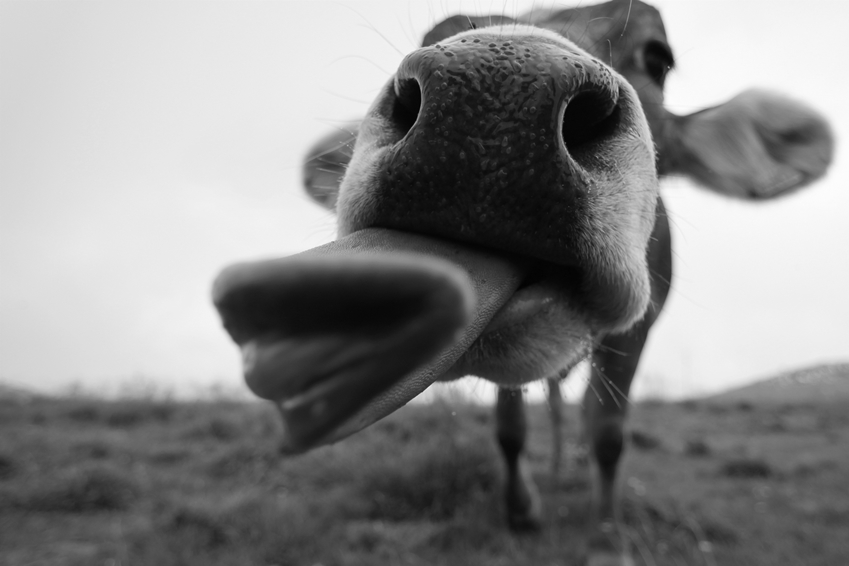
\includegraphics[width=0.9\textwidth]{03_GraphicFiles/CowLickingNose.jpg}
	\captionsource{A cow licking its nose. Usage with permission of the photographer \textsc{Nicole Barth}}{Obtenido de \url{www.flickr.com/photos/46311827@N07/14885545396}, (2017)}
	\label{fig:CowLickingNose}
\end{figure}


%\plotFile{x}{y}{07_DataForPlot/ej-data-plot.txt}
\begin{figure}[htb]
	\centering
	\begin{tikzpicture}
	\begin{axis}[unit vector ratio=1 1 % same size for both unit axis vectors
				, ylabel={Correct Codes}
				, ylabel style= {yshift=-4mm,}
				, xlabel={Keyword Frequency (Code)}
				, width = 0.9\textwidth
				, height= 80mm
				, cycle list name=Dark2
				, grid=major
				, legend pos=outer north east
				, legend style= {cells={anchor=west}, outer ysep=0pt}
				, xmin=0
				, xmax=11.5
				, ymin=0
				, every axis plot post/.style={very thick}
				, grid style=dashed
				, title style={font=\bfseries,align=center,text width=0.7\textwidth}
				, title = {Diagrama de ejemplo}
				]

\addplot+[smooth, mark=*] coordinates {(1,5)(2,5)(3,4)(4,5)(5,5)(6,5)(7,5)(8,5)(9,5)(10,5)};
\addplot+[smooth, dashed, mark=square*, mark options={solid}] coordinates {(1,9)(2,6)(3,6)(4,5)(5,4)(6,5)(7,6)(8,5)(9,5)(10,5)};
\addplot+[smooth, dotted, mark=triangle*, mark options={solid}] coordinates {(1,6)(2,7)(3,7)(4,6)(5,7)(6,9)(7,10)(8,10)(9,9)(10,9)};
\addplot+[smooth, densely dashed, mark= diamond*, mark options={solid}] coordinates {(1,7)(2,6)(3,5)(4,5)(5,7)(6,4)(7,4)(8,4)(9,4)(10,5)};

\legend{WordCount,KeywordRelevance,KeywordCount,DISCOKeywords}
\end{axis}
\end{tikzpicture}
\captionsource{Plot realizado con Tikz usando como colores Dark2}{\fuentePropia}
\label{fig:plot-example}
\end{figure}

\section{Ecuaciones}
\label{sec:equations}
This is how a equation looks like in this document:

\begin{equation}
\cos (2\theta) = \cos^2 \theta - \sin^2 \theta
\end{equation}

\begin{equation}
	F1 = \frac{2 \cdot Precision\cdot Recall}{Precision+ Recall}
\end{equation}

\begin{equation}
	Precision = \frac{TP}{TP+ FP}
\end{equation}

\begin{equation}
	Precision = \frac{\big[\big\{documentos \ relevantes\big\} \cap \big\{documentos \ recuperados\big\}\big]}{\big\{documentos \ recuperados\big\}}
\end{equation}

\begin{equation}
	Recall = \frac{TP}{TP+ FN}
\end{equation}

\begin{equation}
	Recall = \frac{\big[\big\{documentos \ relevantes\big\} \cap \big\{documentos \ recuperados\big\}\big]}{\big\{documentos \ relevantes\big\}}
\end{equation}

\section{Algoritmos}

\begin{algorithm}[hbt]
	\caption{Escribiendo algoritmos usando \LaTeX2e}
	\SetAlgoLined
	\KwIn{Esto es la entrada del algoritmo}
	\KwOut{Esto es la salida del algoritmo}
	%\KwData{Esto son los datos con que trabaja el algoritmo}
	%\KwResult{Esto es el resultado del algoritmo}
\Begin{
	$V \longleftarrow U$\;
	$S \longleftarrow \emptyset$\;

	\While{not at end of this document}{
		read current\;
		\eIf{understand}{
			go to next section\;
			current section becomes this one\;
		}{
			go back to the beginning of current section\;
		}
	}
}	
\end{algorithm}

\section{Citas}

Para citar ocupar la siguiente forma: 

\begin{itemize}
	\item \cite{Codishetal2000}.
	\item Ej: \textcite{Codishetal2000} menciona que.
\end{itemize}

La bibliografía saldrá dependiendo del tipo de documento citado.

\begin{description}
	\item[Articulo de revista] Iniciales y Apellido del autor, "Título del artículo entre comillas," \textit{Título abreviado de la revista en cursiva}, volumen (abreviado vol.), número abreviado no.), páginas (abreviado pp.), Mes, Año.
	\item[Monografía] Iniciales y Apellido, \textit{Título del libro en cursiva}, Edición. Lugar de publicación: Editorial, Año de publicación.
	\item[Manual técnico] \textit{Título en cursiva del manual}, Edición. Nombre de la empresa, Sede de la empresa, Año de publicación.
	\item[Informes técnicos] Iniciales y Apellido del Autor, "Título del informe entre comillas," Nombre de la empresa, Sede de la empresa, Tipo de informe abreviado, Número de informe, Fecha de publicación.
	\item[Capítulo de un libro] Iniciales y Apellido del Autor, "Título del capítulo entre comillas,". en \textit{Título del libro en cursiva}, Iniciales y Apellido del Editor, Compilador. etc. Editorial: Lugar de publicación, Año de publicación, Páginas (abreviadas pp.)
	\item[Artículo de revista] Iniciales y Apellido del autor, "Título del artículo entre comillas", \textit{Título abreviado de la revista en cursiva}, volumen (abreviado vol.), número abreviado no.), páginas (abreviado pp.), Mes, Año
	\item[Recurso de Internet] Igual que los documentos impresos, añadiéndoles la indicación [online] y el DOI (Digital Object Identifier), que generalmente se corresponde con la URL.
	\item[Documentos ineditos] Iniciales y Apellido del autor, "Título entre comillas," Clase de documento (tesis doctoral, trabajo fin de carrera...), Departamento, Institución académica, Ciudad, Año
\end{description}




\section{Gantt}


\begin{figure}[H]
\centering
\label{tabla:estado-avance}
\scalebox{0.9} {
\begin{ganttchart}[
	today=4
	]{1}{19}
	
	\gantttitle{Proyecto tesis}{19}\\
	\gantttitle[]{2017}{19} \\               
	
	\gantttitle{Mar}{4}                     
	\gantttitle{Abr}{4}
	\gantttitle{May}{4}
	\gantttitle{Jun}{4}
	\gantttitle{Jul}{3} \\ % Fin: Entrega 12 julio 2017
	
	\ganttgroup[inline=false]{Diseño de la arquitectura}{1}{8} \\ 
	\ganttbar[progress=70,inline=false]{Fase de pruebas}{1}{8} \\
	
	\ganttgroup[inline=false]{Diseño de algoritmo de planificación}{1}{19} \\ 
	\ganttbar[progress=50,inline=false]{Evaluación de los algoritmos}{1}{16} \\
	\ganttbar[progress=40,inline=false]{Obtención de resultados}{1}{16} \\
	\ganttbar[progress=40,inline=false]{Generación de gráficos}{1}{16} \\
	\ganttbar[progress=30,inline=false]{Comparación de resultados}{12}{19} \\
	\ganttbar[progress=20,inline=false]{Obtener conclusiones del trabajo}{16}{19} \\
	
	\ganttgroup[progress=70, inline=false]{Redacción del documento}{1}{19} \\ 
\end{ganttchart}	
}
\captionsource{Carta Gantt propuesta.}{\fuentePropia}
\end{figure}



%\section{Destacar cambios}
%Esto es un \correcion{cambio realizado y marcado}.

% Main Part
%%%% File encoding is ISO-8859-1 (also known as Latin-1)
%%% You can use special characters just like ä,ü and ñ

\chapter{Main Part}

\Blindtext[1][1]

\begin{figure}[htb]
\centering
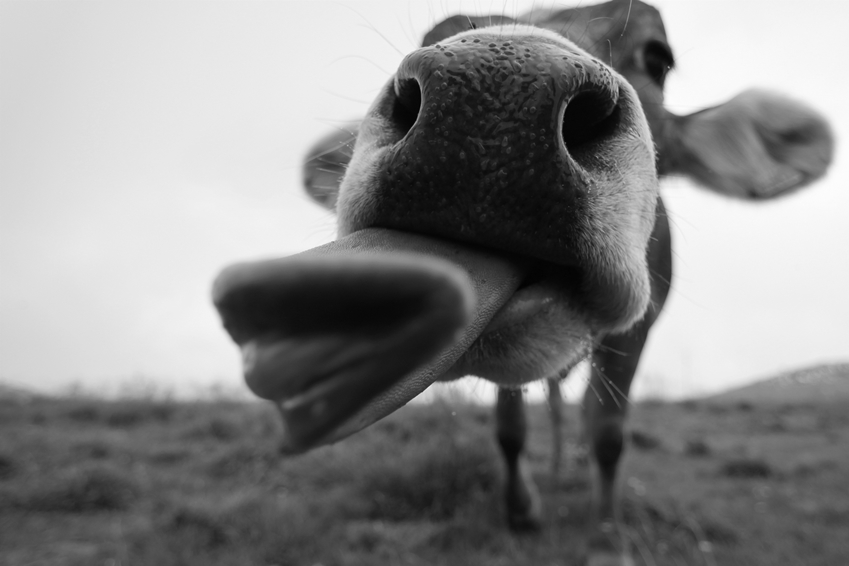
\includegraphics[width=0.9\textwidth]{03_GraphicFiles/CowLickingNose.jpg}
\captionsource{A cow licking its nose. Usage with permission of the photographer \textsc{Nicole Barth}}{Obtenido de \url{www.flickr.com/photos/46311827@N07/14885545396}, (2017)}
\label{fig:CowLickingNose}
\end{figure}

En la \figurename~\ref{fig:CowLickingNose}\myMarginnote{Reference to a figure} you see a cow that is licking its nose. The picture was taken by Nicole Barth on 11.08.2014 using a Canon EOS 500D. The original file has a resolution of $4247 \times 2831$ pixels\footnote{hola como te va}.


\begin{figure}[htb]
\centering
\begin{tikzpicture}
\begin{axis}[
axis lines = middle,
enlargelimits = true,
xlabel = {$x$},
ylabel = {$y$},
trig format plots = rad,
width = 0.9\textwidth,
height= 80mm,
title style={font=\bfseries,align=center,text width=0.7\textwidth},
title = {Example Diagram with a Line Break in the Title (using the \texttt{text width} option in the \texttt{title style})},
]
\addplot[myColorMainA,domain=0:9, line width=1pt, smooth]
{0.2*x^2};
\addplot[myColorMainB,domain=0:9, line width=1pt, smooth]
{5*sin(x)};
\end{axis}
\end{tikzpicture}
\captionsource{A scientific diagram using the \texttt{pgfplots} package by \textsc{Christian Feuersaenger} using the same colors which are also used for the layout}{Elaboración propia, (2017)}
\label{fig:ScientificDiagram}
\end{figure}

\Blindtext[2][2]

\begin{table}[htb]
\centering
\captiontable{A small table created with the \texttt{booktabs} package (example taken from the package documentation).}{Elaboración propia, (2017)}

\begin{tabular}{@{}llr@{}} \toprule
\multicolumn{2}{c}{Item} \\ \cmidrule(r){1-2}
Animal & Description & Price (\$)\\ \midrule
Gnat & per gram & 13.65 \\
& each & 0.01 \\
Gnu & stuffed & 92.50 \\
Emu & stuffed & 33.33 \\
Armadillo & frozen & 8.99 \\ \bottomrule
\end{tabular}

\end{table}


\Blindtext[2][1]

\section{Example Section}

\Blindtext[3][2]

\blinditemize

\section{Another Example Section}

\Blindtext[3][1]

\blindenumerate

\subsection{Example Sub-Section}

\blindmathpaper

\begin{figure}[htb]
\centering
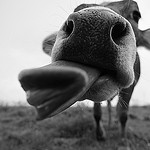
\includegraphics[]{03_GraphicFiles/CowLickingNoseSquare.jpg}
\captionsource{A cow licking its nose -- picture in square format in a native (low) resolution $150 \times 150$ pixels @ 72~dpi ($\approx 2.1$ inch). No scaling in \LaTeX{} using options in \texttt{\textbackslash includegraphics} is applied. Zoom in and see how ugly this is. See \figurename~\ref{fig:CowLickingNose} for reference.}{Elaboración propia, (2017)}
\label{fig:CowLickingNoseSquare}
\end{figure}

\subsection{Another Example Sub-Section}

\Blindtext[2][1]

\subsubsection*{Another Sub-Sub-Section}

\blindmathpaper

\paragraph{Example Paragraph}

\Blindtext[2][1]

\subparagraph{Example Sub-Paragraph}

\Blindtext[2][1]

\section{Yet Another Example Section}

\Blindtext[2][1]

% Final Thoughts
%%%% File encoding is UTF8
%%% You can use special characters just like ä,ü and ñ

\chapter{Final Thoughts}

\textquote[citation]{This is an incomplete sentence}.


%\Blindtext[2][1]

\printbibliography 
% Start appendix
\appendix

% Appendix A
%%% File encoding is UTF8
%%% You can use special characters just like ä,ü and ñ

\chapter{Capítulo Apéndice}



\section{Sección del apéndice}


\centering
\begin{neuralnetwork}[height=4]
	\newcommand{\nodetextclear}[2]{}
	\newcommand{\nodetextx}[2]{$x_#2$}
	\newcommand{\nodetexty}[2]{$y_#2$}
	\inputlayer[count=4, bias=false, title=Input\\layer, text=\nodetextx]
	\hiddenlayer[count=5, bias=false, title=Hidden\\layer, text=\nodetextclear] \linklayers
	\outputlayer[count=3, title=Output\\layer, text=\nodetexty] \linklayers
\end{neuralnetwork}

\begin{figure}[htb]
	\centering
	\begin{tikzpicture}
	\begin{axis}[axis lines = middle
	, enlargelimits = true
	, xlabel = {$x$}
	, ylabel = {$y$}
	, trig format plots = rad
	, width = 0.9\textwidth
	, height= 80mm
	, cycle list name=Dark2
	, title style={font=\bfseries,align=center,text width=0.7\textwidth}
	, title = {Example Diagram with a Line Break in the Title (using the \texttt{text width} option in the \texttt{title style})},
	]
	\addplot[myColorMainA,domain=0:9, line width=1pt, smooth]
	{0.2*x^2};
	\addplot[myColorMainB,domain=0:9, line width=1pt, smooth]
	{5*sin(x)};
	\end{axis}
	\end{tikzpicture}
	\captionsource{A scientific diagram using the \texttt{pgfplots} package by \textsc{Christian Feuersaenger} using the same colors which are also used for the layout}{\fuentePropia}
	\label{fig:ScientificDiagram}
\end{figure}

\subsection{Subseccion del apéndice}

% Appendix B
%%% File encoding is UTF8
%%% You can use special characters just like ä,ü and ñ

\chapter{Another Appendix Chapter}


%TODO: fix with cref
%Como se puede apreciar en la \cref{tab:b1}.
Como se puede apreciar en la \tab{tab:b1}.


\insertTableFile{Ejemplo de una tabla.}{Elaboración propia, (2017)}{04_Tables/CSVexample.csv}{\label{tab:b1}}

\end{document}
% ------------------------------------------------------------------
%
% #######################
% End: Document
% #######################
